\section{\content{注音符號、漢語拼音簡介}{汉语拼音、注音符号简介}}\label{section:bopomofo-pinyin}
\subsection{\content{背景知識}{背景知识}}
\content{回想一下,在你幼時初學漢語(如果你的母語是漢語)的過程中,你是否有過「能認得某個字,但就是不會寫」的經歷?你也可以問問身邊常用漢語的朋友們,他們是否常常提筆忘字?}{回想一下,在你幼时学习汉语(如果你的母语是汉语)的过程中,你是否有过“能认得某个字,但就是不会写”的经历?你也可以问问身边常用汉语的朋友们,他们是否常常提笔忘字?}\par
\content{這樣的情況並不鮮見,因為語言習得的正常規律是從「聽」和「說」開始的。當我們開始學寫字時,其實我們早就會唸不少字了;每學一個新字時,我們也總會更關注它的讀音,而不是寫法。}{这样的情况并不鲜见,因为语言习得的正常规律是从“听”和“说”开始的。当我们开始学写字时,其实我们早就会念不少字了;每学一个新字时,我们也总会更关注它的读音,而不是写法。}\par
\content{我們判斷自己是否「認識」某個字,往往也要以「是否會唸」作為依據。舉些例子,「{\bf 柃}木」「{\bf 囿}於」「虎{\bf 兕}」「{\bf 朊}粒」「{\bf 旻}天」中的五個粗體字,簡單到只要让人看過一眼就會寫了,但是你真的認得它們嗎?與之相反,對於「食{\bf 鹽}」「{\bf 黎}明」「{\bf 罐}頭」「{\bf 贏}家」中的四个粗體字,我們未必都會寫(或許正是人們提筆忘字的範例),但是我們只要看上一眼就可以確信,我們認識這些字!}{我们判断自己是否“认识”某个字,往往也要以“是否会念”作为依据。举些例子,“{\bf 柃}木”“{\bf 囿}于”“虎{\bf 兕}”“{\bf 朊}粒”“{\bf 旻}天”中的五个粗体字,简单到只要让人看过一眼就会写了,但是你真的认得它们吗?与之相反,对于“扫{\bf 帚}”“{\bf 黎}明”“{\bf 罐}头”“{\bf 赢}家”中的四个粗体字,我们未必都会写(或许正是人们提笔忘字的范例),但是我们只要看上一眼就可以确信,我们认识这些字!}\par
\content{可見,我們對「字音」的印象要比對「字形」深得多,所以在學習任何字時,掌握其讀音都是很有必要的。就書面注音而言,現代人一般使用注音符號或漢語拼音來為漢字注音,而古人則使用反切等方法為漢字注音。本節將對漢語注音方法的發展做簡要介紹。}{可见,我们对“字音”的印象要比对“字形”深得多,所以在学习任何字时,掌握其读音都是很有必要的。就书面注音而言,现代人一般使用汉语拼音或注音符号来为汉字注音,而古人则使用反切等方法为汉字注音。本节将对汉语注音方法的发展做简要介绍。}\par
\subsubsection{\content{同音相注法}{同音相注法}}
\content{試想,如果不能用注音/拼音這樣的記號,我們要怎麼表示一個字的讀音呢?最簡單的方法就是用另一個讀音相同的字來為它注音,這就是同音相注法,或稱直音法。}{试想,如果不能用拼音/注音这样的记号,我们要怎么表示一个字的读音呢?最简单的方法就是用另一个读音相同的字来为它注音,这就是同音相注法,或称直音法。}\par
\begin{wrapfigure}{O}{.5\textwidth}
    \centering
    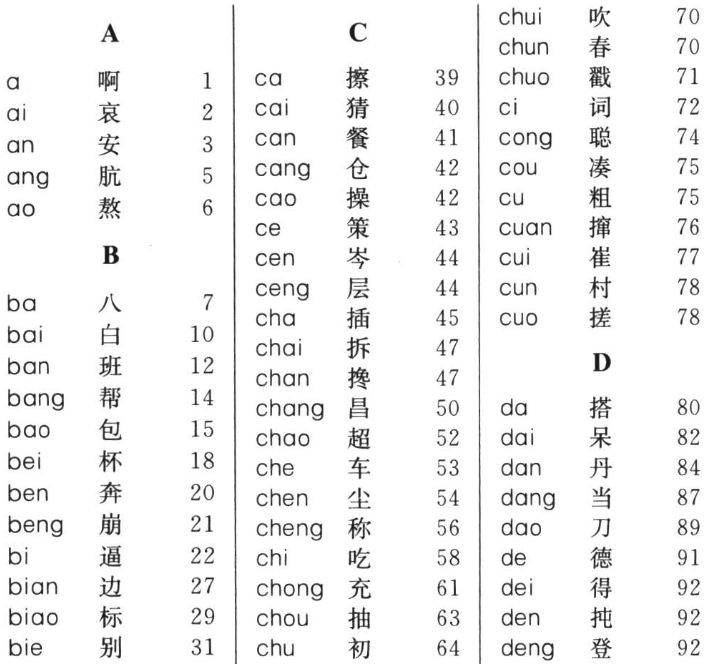
\includegraphics[width=.5\textwidth]{新華字典中的同音相注法.png}
    \caption{\content{新華字典中的音節索引}{新华字典中的音节索引}}
    \label{figure:新華字典中的同音相注法}
    {\footnotesize\color{darkgray} \content{索引中保留了一些同音相注法的痕跡}{索引中保留了一些同音相注法的痕迹}}
\end{wrapfigure}
\content{舉個簡單的例子,如果要為「庵」字注音,我們可以用「安」字。這樣一來,稍有讀音知識的人都可以透過「安」字得知「庵」字的讀音。}{举个简单的例子,如果要为“庵”字注音,我们可以用“安”字。这样一来,稍有读音知识的人都可以通过“安”字得知“庵”字的读音。}\par
\content{《新華字典》的音節索引頁中既有拼音,又有對應拼音的例字(圖\ref{figure:新華字典中的同音相注法})。我們可以認為這是某種意義上的「同音相注」:比如,與「安」同音的字在第三頁。}{《新华字典》的音节索引页中既有拼音,又有对应拼音的例字(图\ref{figure:新華字典中的同音相注法})。我们可以认为这是某种意义上的“同音相注”:比如,与“安”同音的字在第三页。}\par
\content{但是,同音相注法的缺陷也是顯而易見的:如果一個人連常用的漢字都認不全,那他就很難透過已有的讀音知識來判斷新漢字的讀音了。}{但是,同音相注法的缺陷也是显而易见的:如果一个人连常用的汉字都认不全,那他就很难通过已有的读音知识来判断新汉字的读音了。}\par
\content{同音相注法還有其它的尷尬之處。仍以圖\ref{figure:新華字典中的同音相注法}為例,我們看「岑」字,這並不是一個常用字,很多人不認得它。然而,同讀音(\pinyin{cen}\ ㄘㄣ)之下已沒有更常用的字,我們要想同音相注的話,根本找不到合適的選擇!}{同音相注法还有其它的尴尬之处。仍以图\ref{figure:新華字典中的同音相注法}为例,我们看“岑”字,这并不是一个常用字,很多人也不认得它。然而,同读音(\pinyin{cen}\ ㄘㄣ)之下已没有更常用的字,我们要想同音相注的话,根本找不到合适的选择!}\par
\subsubsection{反切法}
\content{反{\bf 切}\textsuperscript{千介切}法在古漢語注音系統中有著舉足輕重的地位。它的基本思路是「二字注一字」:取第一字(上字)的聲母和第二字(下字)的韻母及音調\footnote{這樣說不太準確。關於音調,準確的說法是「陰陽判於上字,平仄斷乎下字」,即上下二字共同決定音調。然而,古今音調規則相差很大,本書無意在此處細究,故正文不提。},拼合起來就是所求之字(歸字)的讀音。}{反{\bf 切}\textsuperscript{千介切}法在古汉语注音系统中有着举足轻重的地位。它的基本思路是“二字注一字”:取第一字(上字)的声母和第二字(下字)的韵母及音调\footnote{这样说不太准确。关于音调,准确的说法是“阴阳判于上字,平仄断乎下字”,即上下二字共同决定音调。然而,古今音调规则相差很大,本书无意在此处细究,故正文不提。},拼合起来就是所求之字(归字)的读音。}\par
\begin{wrapfigure}{O}{.4\textwidth}
    \centering
    \vspace{-2em}
    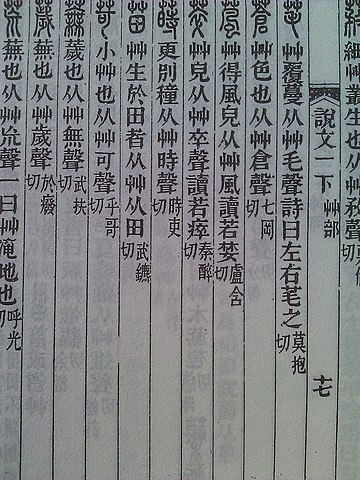
\includegraphics[width=.4\textwidth]{說文-艸部.jpeg}
    \caption{\content{大徐本《說文》草部}{大徐本《说文》草部}}
    \label{figure:說文-艸部}
    {\footnotesize\color{darkgray}\content{圖片來源:維基共享資源}{图片来源:维基共享资源}}
\end{wrapfigure}
\content{方才文中標粗的「切」字是用「千」「介」二字來注音的,我們在拼讀「切」字時,只需取上字「千」的聲母「\pinyin{q}\ ㄑ」和下字「介」的韻調「\pinyin{ie4}\ ㄧㄝˋ」就可以拼出「切」的字音「\pinyin{qie4}\ ㄑㄧㄝˋ」了。}{方才文中标粗的“切”字是用“千”“介”二字来注音的,我们在拼读“切”字时,只需取上字“千”的声母“\pinyin{q}\ ㄑ”和下字“介”的韵调“\pinyin{ie4}\ ㄧㄝˋ”就可以拼出“切”的字音“\pinyin{qie4}\ ㄑㄧㄝˋ”了。}\par
\content{反切注音比同音相注靈活得多,比如「岑」字可以用「才」「人」二字切出,這樣就能在一定程度上避免同音相注法「無字可注」的尷尬。}{反切注音法比同音相注灵活得多,比如“岑”字可以用“才”“人”二字切出,这样就能在一定程度上避免同音相注法“无字可注”的尴尬。}\par
\content{更重要的是,反切對於語音系統的分析更為透徹。從反切開始,人們已經有了完善的聲韻觀念和系統化的拼讀規則。一個人只需認得一些常見的反切上下字,就可以拼讀任何注音文字。東漢以後,反切法大行其道,無論韻書、辭典,無一不用反切注音(圖\ref{figure:說文-艸部})。}{更重要的是,反切对于语音系统的分析更为透彻。从反切开始,人们已经有了完善的声韵观念和系统化的拼读规则。一个人只需认得一些常见的反切上下字,就可以拼读任何注音文字。东汉以后,反切法大行其道,无论韵书、辞典,无一不用反切注音(图\ref{figure:說文-艸部})。}\par
\subsubsection{\content{威妥瑪拼音}{威妥玛拼音}}
\content{威妥瑪拼音(Wei\textsuperscript{1}\ T'o\textsuperscript{3}-ma\textsuperscript{3}\ P'in\textsuperscript{1}-yin\textsuperscript{1})產生於19世紀後半葉,它是使用拉丁字母為漢語注音的較早嘗試,也是19\textasciitilde20世紀期間使用最為廣泛的拉丁注音。}{威妥玛拼音(Wei\textsuperscript{1}\ T'o\textsuperscript{3}-ma\textsuperscript{3}\ P'in\textsuperscript{1}-yin\textsuperscript{1})产生于19世纪后半叶,它是使用拉丁字母为汉语注音的较早尝试,也是19\textasciitilde20世纪期间使用最为广泛的拉丁注音。}\par
\content{在漢語拼音出現後,威妥瑪拼音已經逐漸被漢語拼音所取代。但是,我們仍然可以在部分英譯名中看到威妥瑪拼音的痕跡,比如「北京大學」是「{\bf Peking} University」,「台北」是「{\bf Taipei}」,「太極」是「{\bf Taichi}」,「易經」是「{\bf I Ching}」。這些都是威妥瑪拼音的拼法。}{在汉语拼音出现后,威妥玛拼音已经逐渐被汉语拼音所取代。但是,我们仍然可以在部分英译名中看到威妥玛拼音的痕迹,比如“北京大学”是“{\bf Peking} University”,“台北”是“{\bf Taipei}”,“太极”是“{\bf Taichi}”,“易经”是“{\bf I Ching}”。这些都是威妥玛拼音的拼法。}\par
\content{威妥瑪拼音是用來拼讀現代標準漢語的,它與注音符號、漢語拼音之間有較好的對應關係。威妥瑪拼音的使用時間相當長,直到2010年台灣在仍廣泛使用。}{威妥玛拼音是用来拼读现代标准汉语的,它与注间符号、汉语拼音之间有较好的对应关系。威妥玛拼音的使用时间相当长,直到2010年台湾仍在广泛使用。}\par
\begin{wrapfigure}{I}{.4\textwidth}
    \centering
    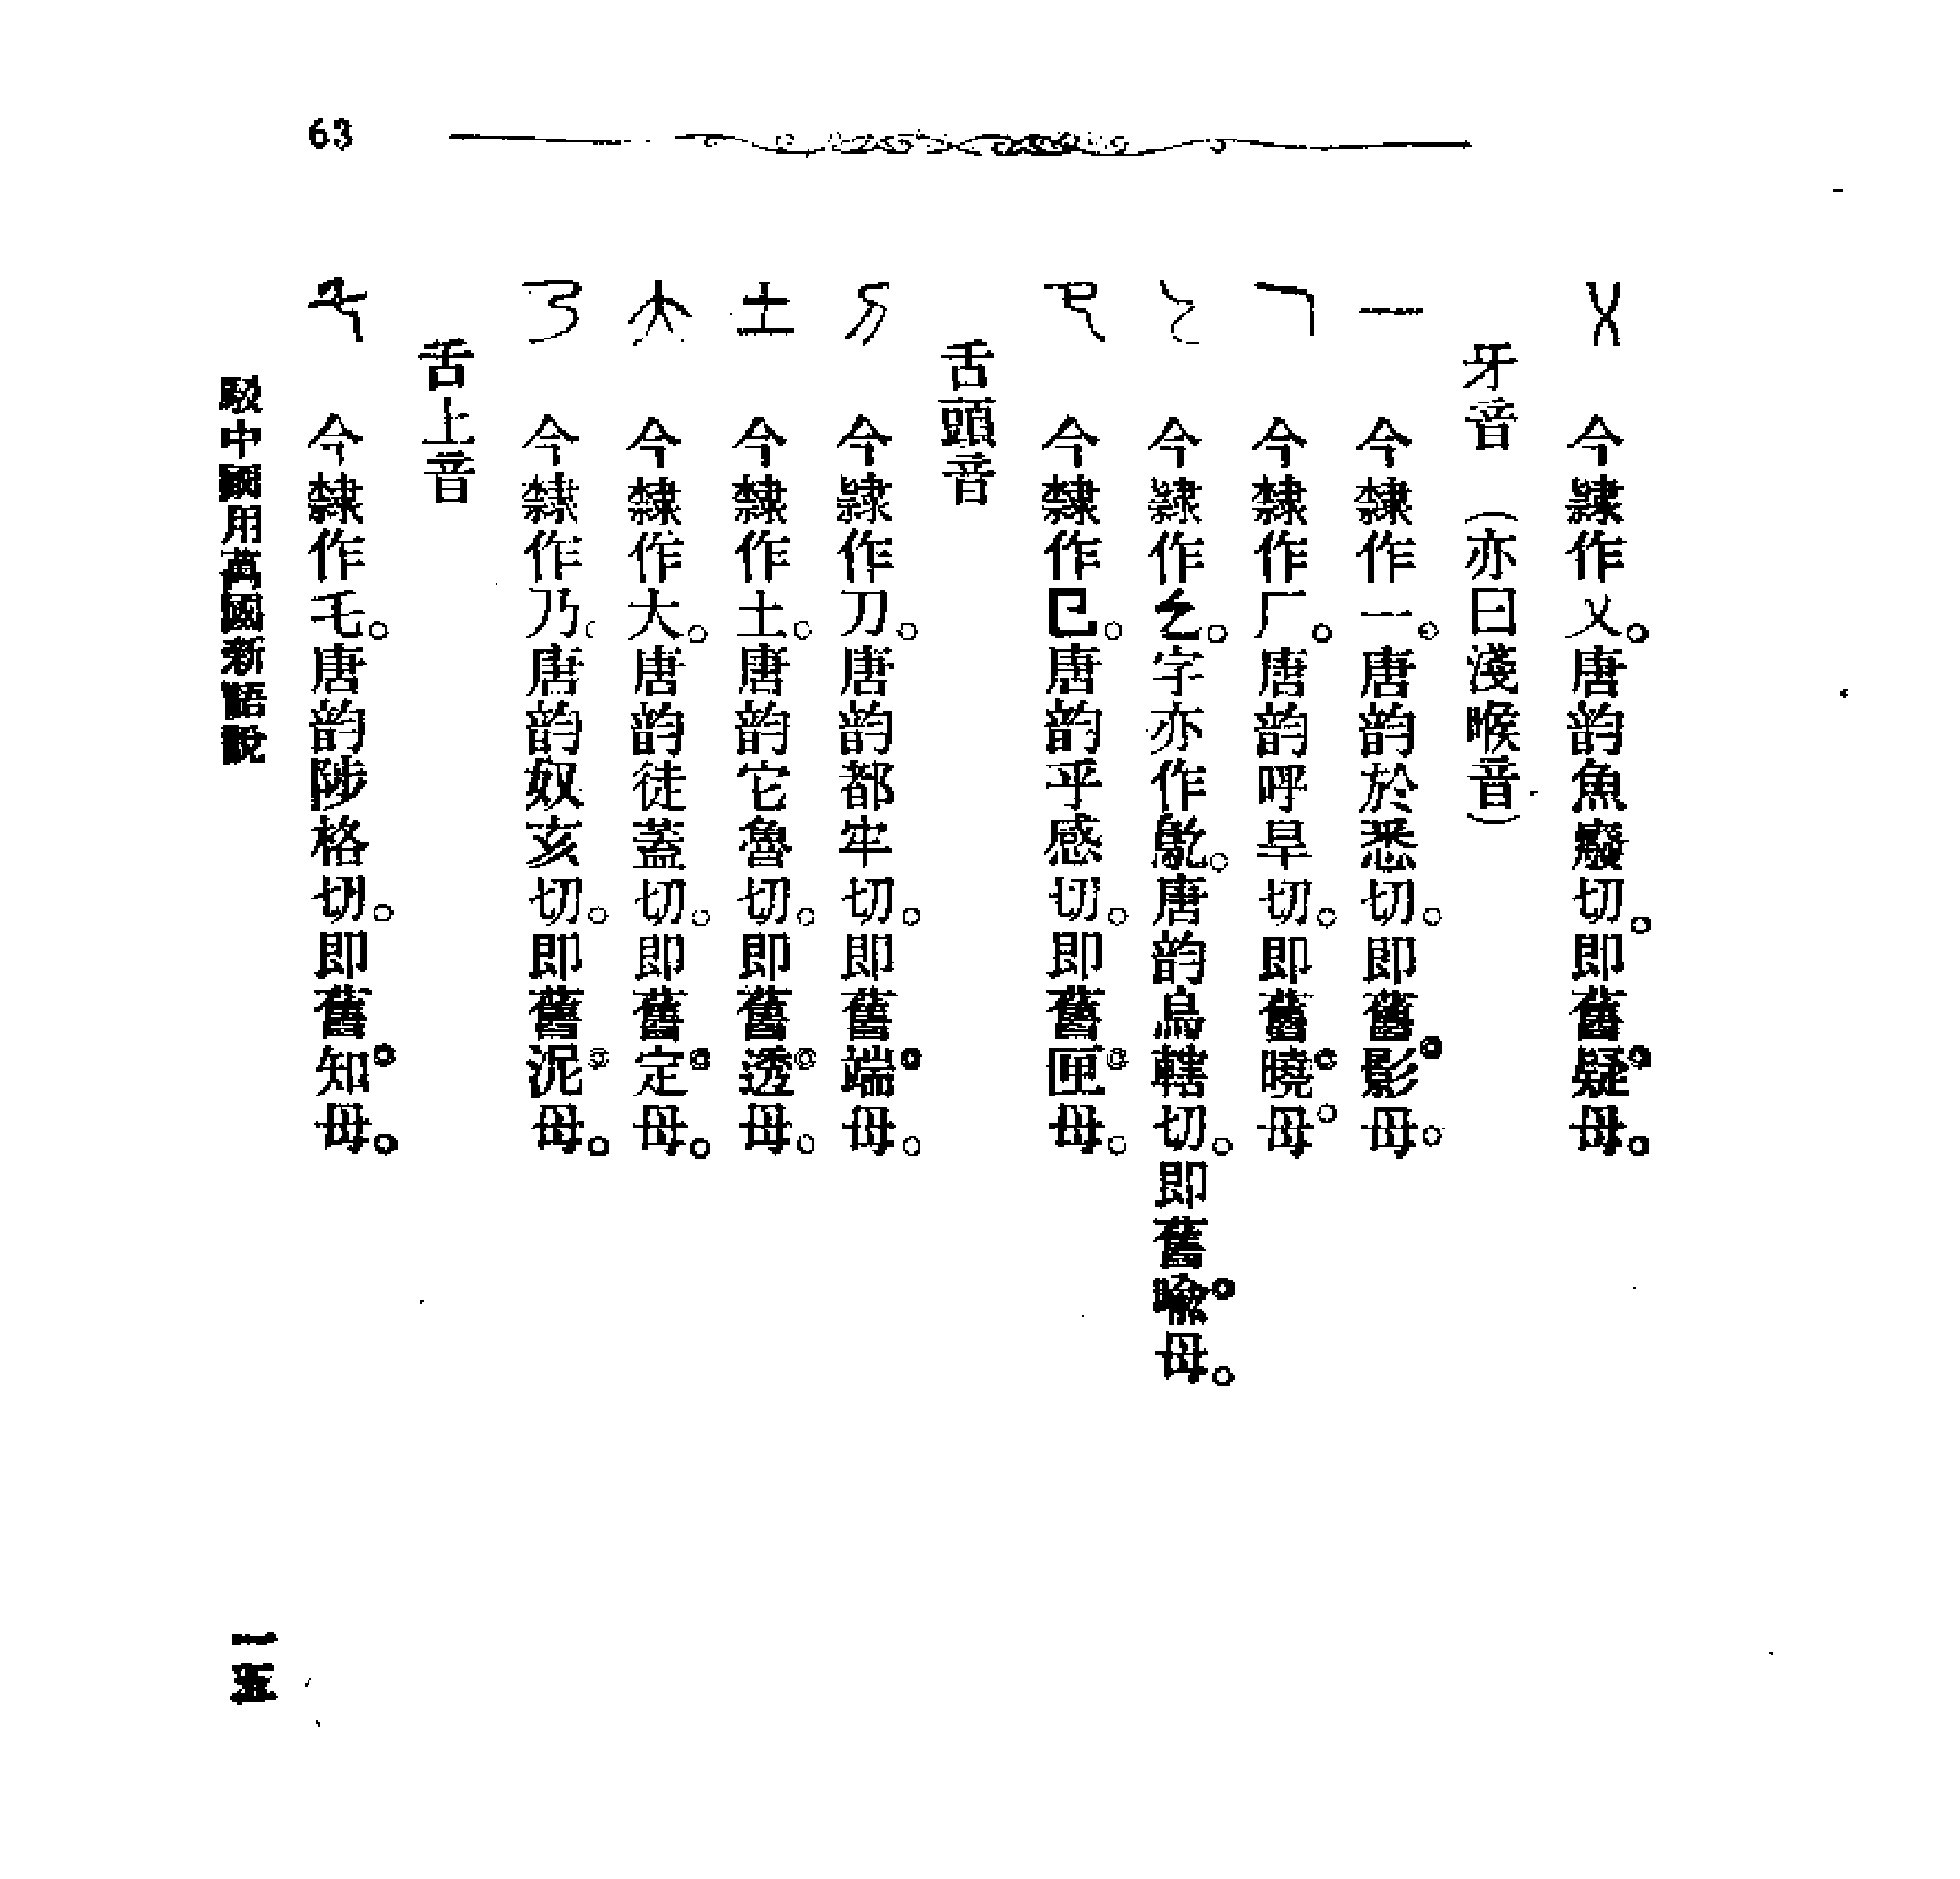
\includegraphics[width=.4\textwidth]{章太炎《駁中國用萬國新語說》「紐文」一頁.png}
    \caption{\content{章太炎《駁中國用萬國新語說》中的一頁,介紹的是紐文}{章太炎《驳中国用万国新语说》中的一页,介绍的是纽文}}
    \label{figure:章太炎《駁中國用萬國新語說》「紐文」一頁}
    {\footnotesize\color{darkgray}\content{《民報》第21號}{《民报》第21号}}
\end{wrapfigure}
\parbox[-1em]{0em}{}
\vspace{-2em}
\subsubsection{\content{注音符號}{注音符号}}
\content{回顧一下前面講到的反切法吧。它的思路是很清晰的:一「聲」一「韻」得一字。但在實際操作中,反切法是用另兩個字分別提供的聲母和韻母來為某個字注音的。按維基大典的說法,反切法需要約四百個上字,約一千個下字,這就要求反切法的使用者先得認識許多字的讀音。而在使用反切法的過程中,我們還需要把上字的聲和下字的韻調分別提取出來再拼合,這個過程也是十分繁瑣的。}{回顾一下前面讲到的反切法吧。它的思路是很清晰的:一“声”一“韵”得一字。但在实际操作中,反切法是用另两个字分别提供的声母和韵母来为某个字注音的。按维基大典的说法,反切法需要约四百个上字,约一千个下字,这就要求反切法的使用者先得认识许多字的读音。而在使用反切法的过程中,我们还需要把上字的声和下字的韵调分别提取出来再拼合,这个过程也是十分繁琐的。}\par
\content{如果我們要重新設計一套拼讀系統的話,自然不難想到,其實我們完全可以自訂一套聲母和韻母,根本沒必要用別的漢字來「反切」聲韻。這也正是清末許多學者努力的方向。}{如果我们要重新设计一套拼读系统的话,自然不难想到,其实我们完全可以自定义一套声母和韵母,根本没必要用别的汉字来“反切”声韵。这也正是清末许多学者努力的方向。}\par
\content{章太炎模仿日語假名的做法,借用漢字的偏旁等部件創造了若干「紐文」「韻文」,這是注音符號的前身(圖\ref{figure:章太炎《駁中國用萬國新語說》「紐文」一頁})。中華民國教育部在章太炎所創方案的基礎上制訂了初代「注音字母」。其後,這套方案又經過歷次修改,終於形成了我們現在看到的「注音符號」。}{章太炎模仿日语假名的做法,借用汉字的偏旁等部件创造了若干“纽文”“韵文”,这是注音符号的前身(图\ref{figure:章太炎《駁中國用萬國新語說》「紐文」一頁})。中华民国教育部在章太炎所创方案的基础止制定了初代“注音字母”。其后,这套方案又经过历次修改,终于形成了我们现在看到的“注音符号”。}\par
\content{現今,注音符號在台灣廣泛使用,也是台灣小學生的必修課。而在中國大陸、香港和澳門,注音符號的使用相對較少。}{现今,注音符号在台湾广泛使用,也是台湾小学生的必修课。而在中国大陆、香港和澳门,注音符号的使用相对较少。}\par
\subsubsection{\xpinyin*{\content{漢語拼音}{汉语拼音}}}
\content{如果說注音符號是「假名派」,仿用假名的思路創造聲符;那麼漢語拼音和威妥瑪拼音一樣,都屬於「拉丁派」,使用拉丁字母來創造聲符。}{如果說注音符號是「假名派」,仿用假名的思路創造聲符;那麼漢語拼音和威妥瑪拼音一樣,都屬於「拉丁派」,使用拉丁字母來創造聲符。}\par
\content{漢語拼音系統始於1950年代,是由王力等語言學家整合早期漢字拉丁化基礎與各種拼音方案而開發出的新拼音方案。相比於威妥瑪拼音等舊方案,漢語拼音易於學習和使用(尤其是節省了許多修飾符),無論手寫還是電腦輸入都十分方便。}{汉语拼音系统始于1950年代,是由五力等语言学家整合早期汉字拉丁化基础与各种拼音方案而开发出的新拼音方案。相比于威妥玛拼音等旧方案,汉语拼音易于学习和使用(尤其是省略了许多修饰符),无论手写还是电脑输入都十分方便。}\par
\content{現今,漢語拼音方案已經成为漢字轉寫為拉丁字母的規範方式,也是國際普遍承認的漢語拉丁轉寫標準。中國大陸和香港、澳門都將漢語拼音作為小學生的必修課;台灣於2008年起开始採用漢語拼音替代威妥瑪拼音和通用拼音\footnote{通用拼音是台灣的本土拉丁字母拼音方案,於2002年推行,但不久後就被漢語拼音所替代。}。}{现今,汉语拼音方案已经成为汉字转写为拉丁字母的规范方式,也是国际普遍承认的汉语拉丁转写标准。中国大陆和香港、澳门都将汉语拼音作为小学生的必修课;台湾于2008年起开始采用汉语拼音替代威妥玛拼音和通用拼音\footnote{通用拼音是台湾的本土拉丁字母拼音方案,于2002年推行,但不久后就被汉语拼音所替代。}。}\par
\subsection{\content{由漢語拼音推導注音符號}{由汉语拼音推导注音符号}}

\subsection{\content{由注音符號推導漢語拼音}{由注音符号推导汉语拼音}}
